%%%%%%%%%%%%%%%%%%%%%%%%%%%%%%%%%%%%%%%%%
% Journal Article
% LaTeX Template
% Version 1.3 (9/9/13)
%
% This template has been downloaded from:
% http://www.LaTeXTemplates.com
%
% Original author:
% Frits Wenneker (http://www.howtotex.com)
%
% License:
% CC BY-NC-SA 3.0 (http://creativecommons.org/licenses/by-nc-sa/3.0/)
%
%%%%%%%%%%%%%%%%%%%%%%%%%%%%%%%%%%%%%%%%%

%----------------------------------------------------------------------------------------
%	PACKAGES AND OTHER DOCUMENT CONFIGURATIONS
%----------------------------------------------------------------------------------------

\documentclass{article}

%\documentclass{aastex}  % version 5.0 or prior
%\usepackage{natbib}



\usepackage{graphicx}
\usepackage{lipsum} % Package to generate dummy text throughout this template
%\usepackage[sc]{mathpazo} % Use the Palatino font
\usepackage[T1]{fontenc} % Use 8-bit encoding that has 256 glyphs
\linespread{1.05} % Line spacing - Palatino needs more space between lines
\usepackage{microtype} % Slightly tweak font spacing for aesthetics

\usepackage[margin=1in,columnsep=20pt]{geometry} % Document margins
\usepackage{multicol} % Used for the two-column layout of the document
\usepackage[hang, small,labelfont=bf,up,textfont=it,up]{caption} % Custom captions under/above floats in tables or figures
\usepackage{booktabs} % Horizontal rules in tables
\usepackage{float} % Required for tables and figures in the multi-column environment - they need to be placed in specific locations with the [H] (e.g. \begin{table}[H])
\usepackage{hyperref} % For hyperlinks in the PDF
\usepackage{subcaption}

\usepackage{lettrine} % The lettrine is the first enlarged letter at the beginning of the text
\usepackage{paralist} % Used for the compactitem environment which makes bullet points with less space between them
\usepackage{amsmath}
\usepackage{abstract} % Allows abstract customization
\renewcommand{\abstractnamefont}{\normalfont\bfseries} % Set the "Abstract" text to bold
\renewcommand{\abstracttextfont}{\normalfont\small\itshape} % Set the abstract itself to small italic text

\usepackage{titlesec} % Allows customization of titles
%\renewcommand\thesection{\Roman{section}} % Roman numerals for the sections
%\renewcommand\thesubsection{\Roman{subsection}} % Roman numerals for subsections
%\renewcommand\thesubsubsection{\Alph{subsubsection}} % Roman numerals for subsections
\titleformat{\section}[block]{\LARGE\scshape}{\thesection}{1em}{} % Change the look of the section titles
\titleformat{\subsection}[block]{\Large\scshape}{\thesubsection}{1em}{} % Change the look of the section titles
\titleformat{\subsubsection}[block]{\large\scshape}{\thesubsubsection}{1em}{} % Change the look of the section titles

\usepackage{fancyhdr} % Headers and footers
\pagestyle{fancy} % All pages have headers and footers
\fancyhead{} % Blank out the default header
\fancyfoot{} % Blank out the default footer
\fancyhead[C]{Montana State University \quad $\bullet$ \quad CSCI 466 Artificial Intelligence \quad $\bullet$ \quad Group 21} % Custom header text
\fancyfoot[RO,LE]{\thepage} % Custom footer text

\newcommand{\ve}[1]{\boldsymbol{\mathbf{#1}}}

\title{\vspace{-15mm}\fontsize{24pt}{10pt}\selectfont\textbf{CSCI 446 Artificial Intelligence \\[2mm] Project 2 Design Report} } % Article title
\date{\today}
\author{
\large
\textsc{Roy Smart} \and \textsc{Nevin Leh} \and \textsc{Brian Marsh}\\[2mm] % Your name
}


%----------------------------------------------------------------------------------------

\begin{document}

	\maketitle % Insert title
	\thispagestyle{fancy} % All pages have headers and footers
	\normalsize

	\section{Introduction}
	
		\textit{Logic and the Wumpus World} is an artificial intelligence problem first proposed by Michael Genesereth, and described in detail by his student Stuart Russel\cite{ai}.  The problem involves navigating an environment known as the Wumpus World using logic to avoid dangers as the agent attempts to reach a goal.  The environment is a square grid of tiles that can be empty or contain gold for the goal state, a pit that the agent will fall into, or a monster known as a wumpus.  As the agent navigates the environment, a score is calculated from the various actions that the agent makes.  The objective of the game is thus to maximize the score, which can be achieved by using logic to find the most efficient route.
	
	\section{Problem Statement}
	
		To solve the Wumpus World problem, we will develop a problem generator that creates the wumpus worlds in which the agent will navigate.  We will then implement a logic system that uses unification and resolution on first-order rules that allow the agent to navigate.  The reasoning system will use the following information: the stench when near a Wumpus, the breeze when near a pit, the scream of a wumpus as it is killed, and the wall when ran into.  Additionally, a reactive agent will be created that makes decisions based upon random decisions regarding which cells are safe and which are not.  We will test the logic system on wumpus worlds of sizes {5x5, 10x10,…, 25x25}.  Our performance metrics are as follows: number of times the gold is found, number of wumpi killed, number of times the explorer falls into a pit, number of times the wumpus kills the explorer, and number of cells explored.
	
	\section{Software Design}
		Our design will incorporate three main classes: \texttt{World}, \texttt{EnvironmentEngine}, and \texttt{Agent}. 
		These classes have all of the important attributes and functions needed to implement this game.
		The \texttt{World} class is responsible for creating and maintaining worlds.
		The \texttt{EnvironmentEngine} is responsible for checking the move an agent selects and then telling the agent the result of the move.
		Finally, the \texttt{agent} is an abstract class that uses information provided by the \texttt{EnvironmentEngine} to decide what the next move is. The three implemented versions of \texttt{Agent} are \texttt{HumanAgent}, \texttt{ReactiveAgent} , and \texttt{ReasoningAgent}.
		
		
		
	
		
		The implementation of the  \texttt{Agent} class is very important. 
		We chose to create an abstract class because we required three unique agents that had some of the same instance variable and methods. Each agent has an agent world variable that is blank except for the starting square initially. 
		This world will be updated as each agent discovers things about the world and according to each agents abilities. 
		The two methods that are shared across agents are \texttt{next\_move} and \texttt{update\_world}. 
		\texttt{next\_move} is used called to see the results of the previous move and returns its choice for the next move. 
		Each agent implements this method in a unique way since each agent determines it's next move differently. 
		The other method, \texttt{update\_world}, is responsible for taking in the result of the previous move and adding it to the knowledge base. 
		The agent can then use this updated world to make the best decision possible. 
		Again, each agent updates the world differently and, therefore, the \texttt{update\_world} method is different for each agent.
		
	
		   \begin{figure}[h!]
		   	\centering
		   	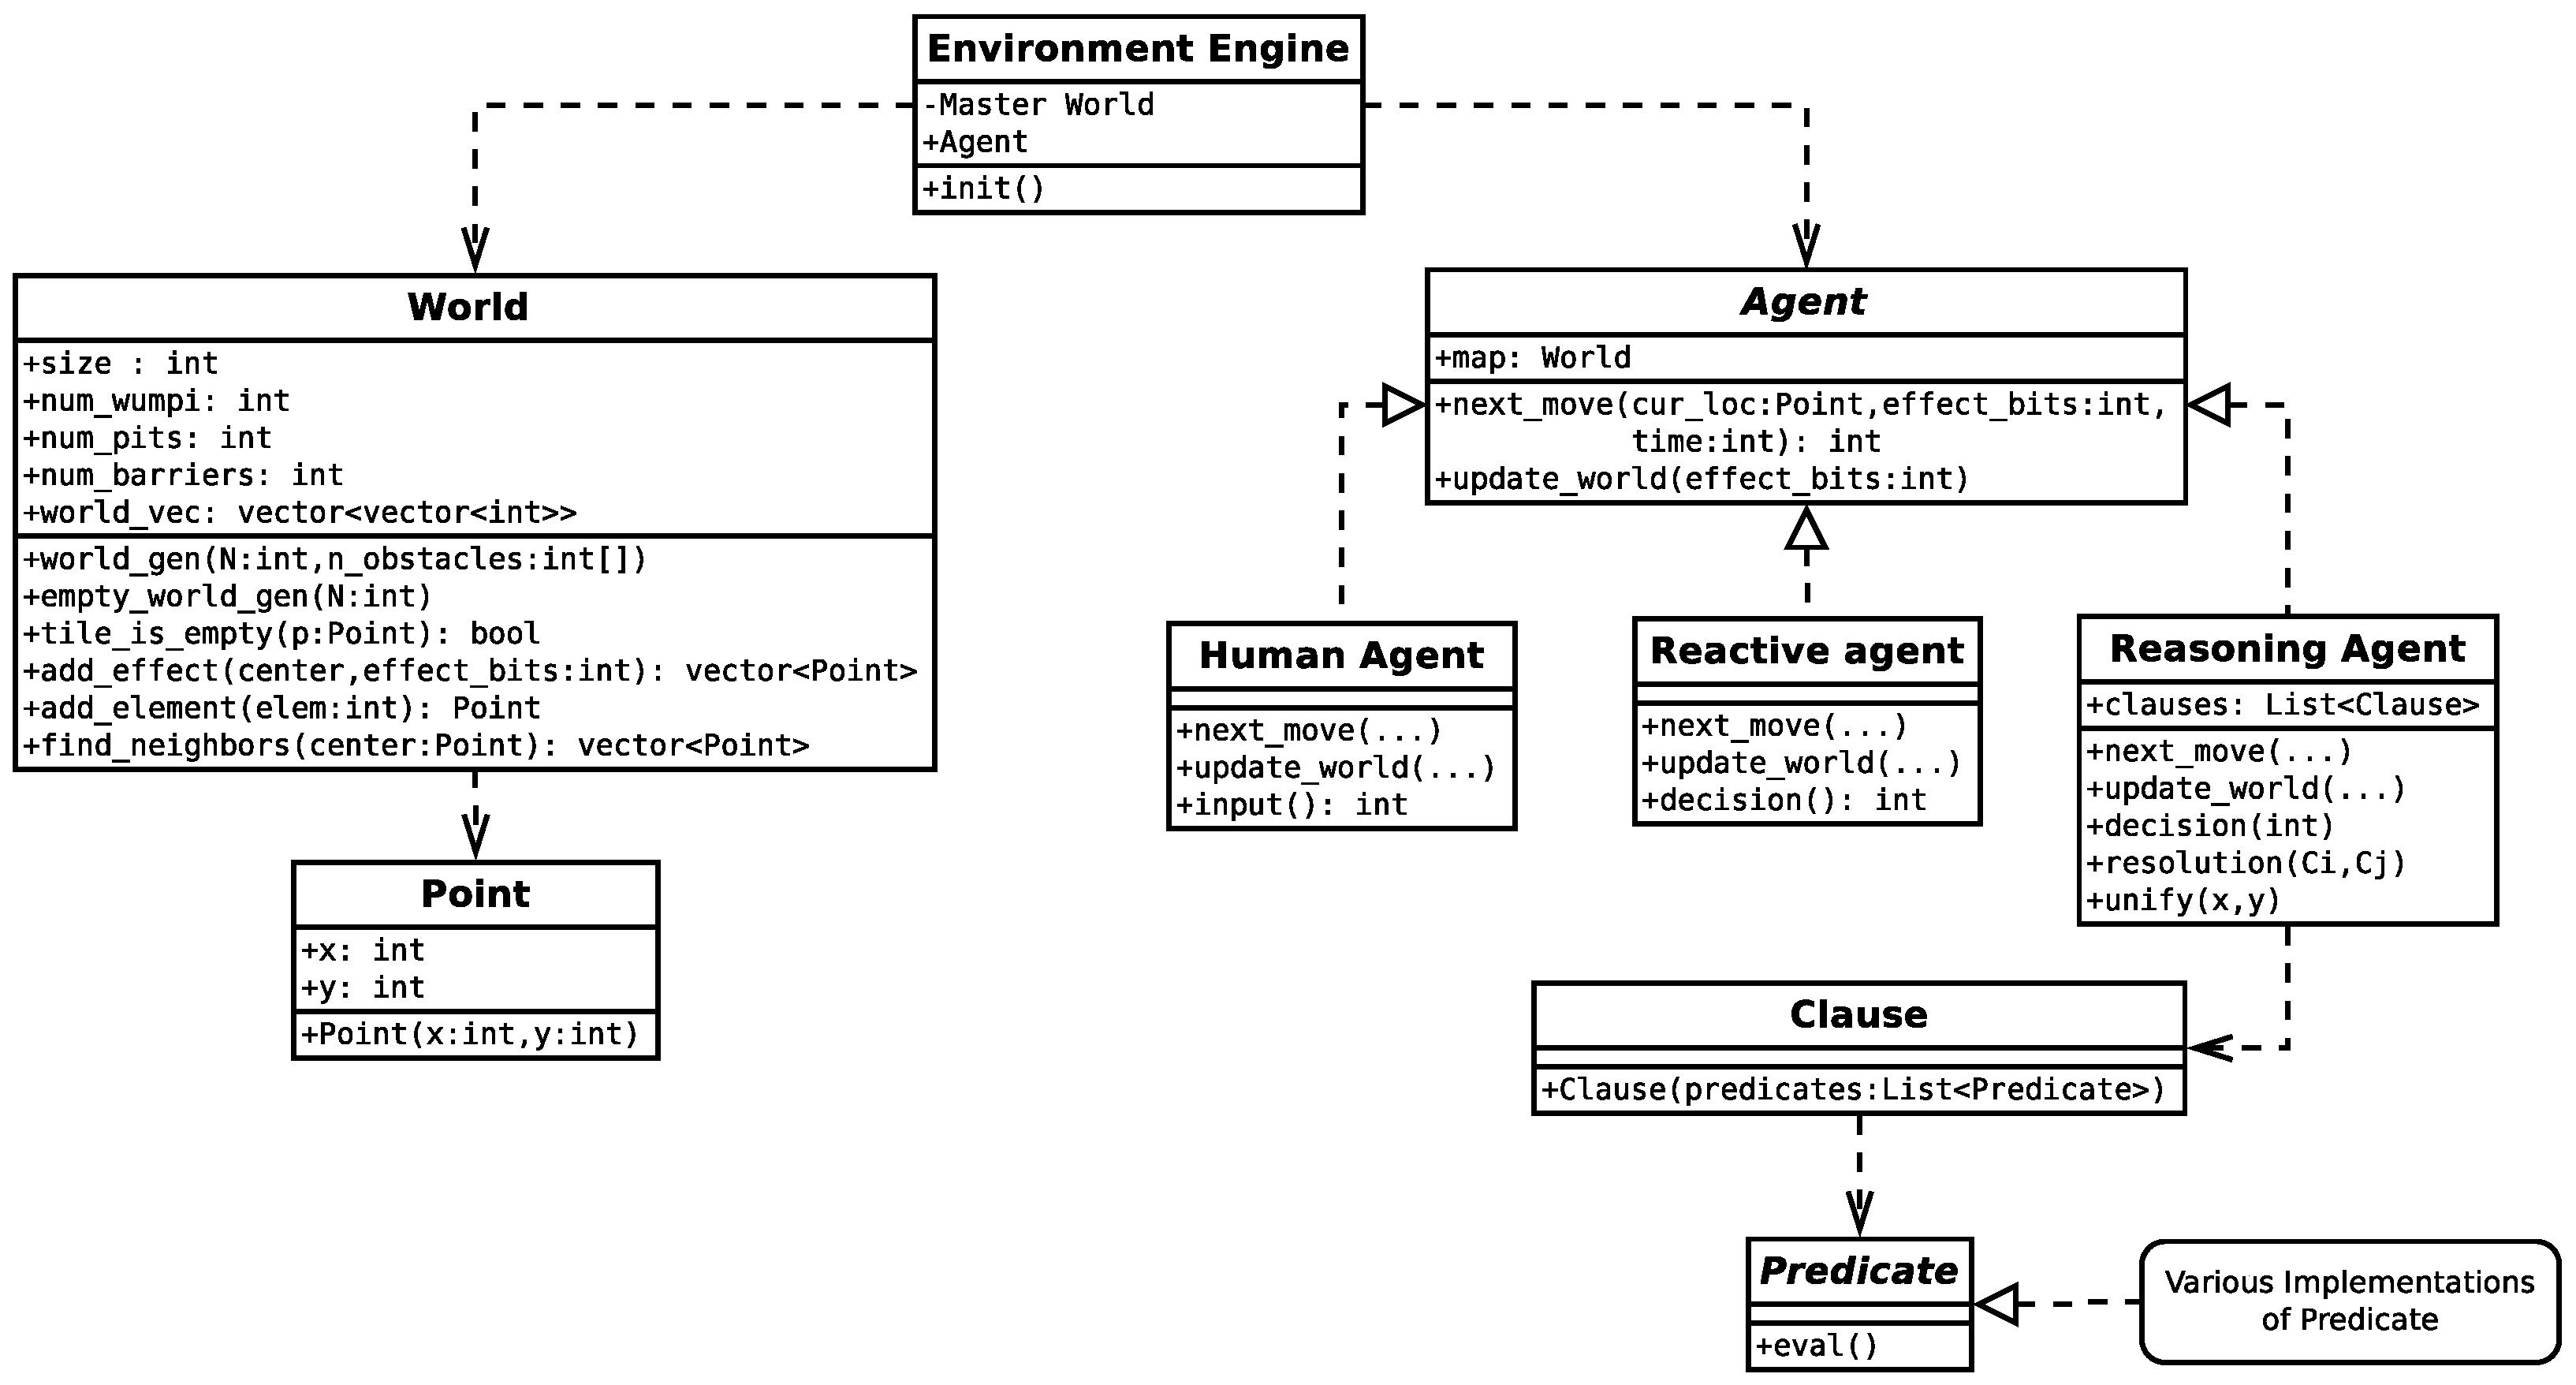
\includegraphics[width = 1\textwidth]{diagrams/uml_project2}
		   	\caption{A UML diagram describing the proposed layout for our program.}
		   	\label{uml}
		   \end{figure}
		
		\subsection{Wumpus World Generation}
		
			The \texttt{World} class is used to create both the fully populated ''Master World`` and the blank ''Agent World``. 
			A world will consist of a vector of vectors that each hold an int.
			Each int represents one square in the world, with each bit representing the presence of a certain feature. 
			We chose to represent the board this way because it seemed more simple than using a whole object for each tile.
			We decided to use a vector of vectors because they are much more forgiving to work with than two dimensional arrays in c++.
			The \texttt{World} class will also be responsible for keeping some important data such as number of wumpi and pits for general usage throughout the program.
		
		\subsection{Environment Engine}
		The \texttt{EnvironmnetEngine} is responsible for holding the master world object and  telling the agents about the world as it is explored.
		It's main job is to operate a loop that constantly calls the \texttt{update\_world} method in the agent. 
		The idea is that the \texttt{update\_world} returns the agents next move. 
		The \texttt{EnvironmentEngine} then applies that move to the master world.
		The next time \texttt{update\_world} is called the \texttt{EnvironmentEngine} includes the results of the attempted move.
		These results include the agents new position, the integer that represents the facts about that square, and miscellaneous facts such as whether a bump was detected. 
		This system is a good option because the same \texttt{EnvironmnentEngine} can be used for all of the agents. 
		\subsection{Reasoning Agent}
		\label{reason}
		
			Our reasoning agent will acquire knowledge about the world around it through its precepts, such as stench, breeze, and bump. These precepts will be inserted into the knowledge base, where the inference engine will use the precepts and logical implications to infer new information that could not be directly perceived (such as the location of the wumpus). The inference engine will only have the ability to answer specific questions, e.g. "Is there a wumpus at this square?" or "Is this square clear?", so our agent will need appropriate control logic to ensure that it queries the correct sequence of questions to the inference engine.  
		
			\subsubsection{Inference Engine}
			\label{inference}
			
				Our inference engine will use the function \textsc{PL-Resolution}($KB$, $\alpha$) described by Russel and Norvig in Figure 7.12 \cite{ai} to perform \textit{resolution}. 
				Resolution allows the inference engine to use a knowledge base of facts to ascertain new details about the wumpus world. 
				The function \textsc{PL-Resolution} accepts a knowledge base, $KB$ and $\alpha$, the query to be checked. Of course, \textsc{PL-Resolution} is based on propositional logic clauses, but according to Section 9.5.2 of Russel and Norvig, we can adapt it to operate using first order logic clauses if we we modify the function \textsc{PL-Resolve($C_i$, $C_j$)} to find two variables complementary if one \textit{unifies} with the negation of the other. 
				
				To check if two variables can be unified, we will use the function \textsc{Unify}($x$, $y$, $\theta$) provided in Figure 9.1 of Russel and Norvig.
				In the interest of efficiency, we will also implement a \textit{predicate indexing}, described in Section 9.2.3 of Russel and Norvig\cite{ai}.
				The predicate index provides \textsc{Unify}() an efficient way to only attempt unification on sentences that are possible to be unified. 
				We will accomplish this by constructing lists of all facts that use a certain predicate, e.g. all facts that contain the predicate $Adjacent(r,s)$ will be placed into a list.
				Then, if \textsc{Unify()} is asked to unify a sentence containing $Adjacent(u,v)$, it will only have to search the list described in the previous sentence instead of the entire knowledge base.
				
			\subsubsection{Knowledge Base}
			
				The knowledge base will be represented using an object-oriented approach.
				We will define a \texttt{Clause} object, that will contain a list of predicates that are assumed to be in a disjuction. The knowledge base will then be characterized by a list of \texttt{Clause}s that similarly are assumed to be in conjunction. 
				The predicates will be represented by a class called \texttt{Predicate}, that will have an ``abstract'' function named \texttt{eval()}.
				Then, to make specific predicates, we will instantiate classes that inherit from \texttt{Predicate} and override the \texttt{eval()} function.
				This structure provides a way to represent logical facts in \textit{conjunctive normal form}(CNF).
				
				Since our knowledge base can only represent sentences in conjunctive normal form, we will need to ensure all of the rules for the wumpus world are expressed in this form.
				To accomplish this, we will create first-order logic rules for the wumpus world in the spirit of Section 8.3.4 in Russel and Norvig.
				We can then convert these rules to CNF using the process described in Section 9.5.1 in Russel and Norvig, or using \textit{Mathematica} if it is acceptable for this project.
				Since all of our rules will be provided in CNF, there will be no reason to do further CNF conversion, as the resolution process produces clauses that are also in CNF.
				
				Each call to the resolution algorithm will use the information in the knowledge base to find new facts about the wumpus world.
				These facts, in turn will be inserted into the knowledge base to be used in further resolution operations.
				As such, the knowledge base will increase in size as the explorer uncovers new information about a particular wumpus world.
				Great care should be taken to ensure that the knowledge base does not grow so large, or become so disorganized that it cannot be searched efficiently.
				A strategy known as predicate indexing has already been described in the second paragraph of Section \ref{inference} and is one example of how searching the knowledge base can be made more efficient.
				Another possible way to make searching the knowledge base more economical is to organize information by location.
				Many of the logical rules in the wumpus world use the $Adjacent(r,s)$ predicate defined in Section 8.3.4 of Russel and Norvig.
				This implies that the facts pertinent to the resolution process are very often in close spatial proximity, so it seems reasonable that the resolution algorithm should resolve clauses with similar spatial locations first.
			
			
			\subsubsection{Pathfinding}
			
				In the previous sections, we have discussed the role of the inference engine in determining whether a square is safe. We propose to also use the inference engine to inform the agent where to move next.
				We will provide the inference engine with a series of logical statements describing the preferences associated with each actuator e.g. "If there is an obstacle in the way, rotate to the right, otherwise move forward." Using these rules, the agent can ask questions such as "Is the best actuator move forward?", "Is the best actuator rotate to the left?", etc. In this way, our agent will be able to explore the map using only the inference engine and the knowledge base.
			
		\subsection{Reactive Agent}
			The next agent to be implemented is the \texttt{ReactiveAgent}. This agent can only act on the information provided by the cell the agent is currently in. In this case the method \texttt{update\_world} will simply use  the information returned by the \texttt{EnvironmentEngine} as the entirety of the world. This agent won't have a whole world. It only knows about the square it is currently in. The implementation of the \texttt{next\_move} method will consist of some simple logical rules such as always choose a safe square if possible.
		
		\subsection{Human Agent}
		 The human agent is the most simple and will be mostly used for debugging purposes. The \texttt{next\_move} method will simply update the world and then use the result of user input to make moves. This Agent will be useful for testing our boards and making sure that everything is set up correctly. The \texttt{update\_world} will apply the results of the previous move to the local agent world. This world is persistent in that old facts are remembered and it can be determined if the agent has been in a square before or not. 
	\section{Experiment Design}
	
	To analyze the performance of our agents, we are asked to vary various parameters of the wumpus World. These parameters include: the size of the board, and the number of wumpi, pits, and barriers. 
	
	
	

	




	%\bibliographystyle{apj}
	\bibliographystyle{unsrt}	
	\bibliography{sources}
\end{document}
